\section{Auswertung}
\label{sec:Auswertung}

        \subsection{Bestimmung des Kontrasts}

            Für verschiedene Polarisationswinkel zwischen 0 und 360° wird die maximale und 
            minimale Intensität aufgenommen und daraus der Kontrast berechnet. 
            Die Werte befinden sich in Tabelle \ref{tab:kontrast}.

            \begin{table}
                \centering
                \caption{Werte zur Kontrastbestimmung für verschiedene Polarisationswinkel.}
                \label{tab:kontrast}
                \begin{tabular}{c c c c c c}
                    \toprule
                    Winkel/° & $I_{min}$/V & $I_{max}$/V & Kontrast\\
                    \midrule
                    0   & 0,94 & 0,77 & 0,100 \\ 
                    15  & 0,71 & 0,5  & 0,173 \\
                    30  & 0,66 & 0,15 & 0,620 \\
                    45  & 0,70  & 0,07 & 0,818 \\
                    60  & 0,89 & 0,15 & 0,700 \\
                    75  & 1,05 & 0,32 & 0,533 \\
                    90  & 1,00 & 0,84 & 0,087 \\
                    105 & 1,65 & 0,76 & 0,369 \\
                    120 & 2,24 & 0,39 & 0,703 \\
                    135 & 2,30 & 0,30  & 0,769 \\
                    150 & 2,00 & 0,40  & 0,667 \\
                    165 & 1,70 & 0,75 & 0,387 \\
                    180 & 1,00 & 0,81 & 0,105 \\
                    195 & 0,47 & 0,28 & 0,253 \\
                    210 & 0,64 & 0,17 & 0,580 \\
                    225 & 0,77 & 0,09 & 0,790 \\
                    240 & 0,77 & 0,12 & 0,730 \\
                    255 & 1,00 & 0,37 & 0,460 \\
                    270 & 1,06 & 0,93 & 0,065 \\
                    285 & 1,69 & 0,76 & 0,380 \\
                    300 & 2,04 & 1,30  & 0,222 \\
                    315 & 1,72 & 1,00    & 0,265 \\
                    330 & 1,74 & 0,50  & 0,554 \\
                    345 & 1,56 & 0,86 & 0,289 \\
                    \bottomrule
                \end{tabular}
            \end{table}

            Der maximale Kontrast liegt bei einem Winkel von 45° vor, sodass diese Einstellung für die 
            weiteren Messungen verwendet wird. 
            In Abb. \ref{fig:kontrast} sind die prozentualen Kontrastwerte gegen den Rotationswinkel aufgetragen.

            \begin{figure}
                \centering 
                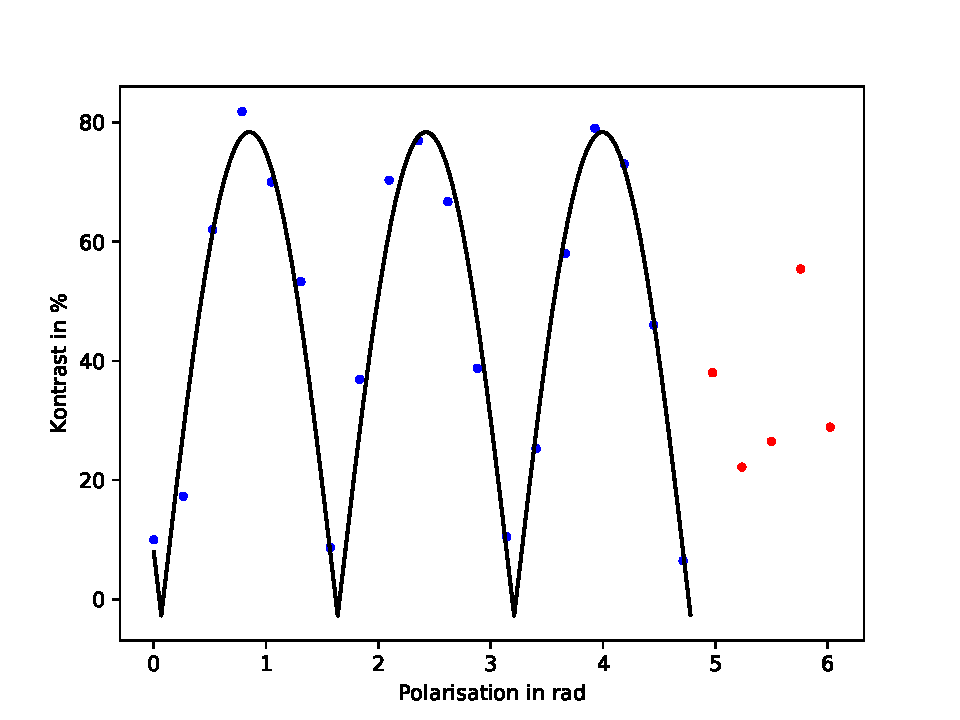
\includegraphics{kontrast.pdf}
                \caption{Fit der polarisationsabhängigen Kontrastwerte.}
                \label{fig:kontrast}
            \end{figure}

            Im Bereich von 0 bis 270° können die Werte mithilfe der Funktion 

            \begin{align*}
                a \cdot \lvert \symup{sin} (2\vartheta+\vartheta_0)\rvert + b
            \end{align*}

            gefittet werden. Dabei ergibt sich für die Parameter

            \begin{align*}
                a &= (81\pm 4)\,\% \\
                b &= (-3\pm 2)\,\% \\ 
                \vartheta_0 &= (-0,1668\pm 0,0003)\,\symup{rad}.
            \end{align*}

            Die letzten Werte zwischen 270 und 360° werden nicht mit in den Fit einbezogen,
            da das Spannungsmessgerät dort stark schwankt und somit keine zuverlässigen 
            Werte für den Kontrast ermittelt werden können.


        \subsection{Bestimmung des Brechungsindexes von Glas}

            Der Brechungsindex von Glas wird mithilfe der Formel 

            \begin{align*}
                n = \frac{1}{1-\frac{M\lambda_{vac}}{2d\theta\theta_0}}
            \end{align*}

            berechnet, wobei $M$ die Anzahl der Maxima, $\lambda_{vac}$ die Wellenlänge des 
            Lasers im Vakuum (632,99\,nm), $d$ die Dicke des Glases (1\,mm), $\theta$ den Drehwinkel (10°)
            und $\theta_0$ den von vornherein gegebenen Drehwinkel (10°) darstellt.
            Die jeweilige Anzahl pro Durchlauf ist in der Tabelle \ref{tab:glas} gegeben. 
            
            \begin{table}
                \centering
                \caption{Anzahl der Maxima in verschiedenen Durchläufen.}
                \label{tab:glas}
                \begin{tabular}{c c c c c c}
                    \toprule
                    Durchlauf & Counts\\
                    \midrule
                        1   & 35 \\
                         2  & 39 \\
                          3 & 36 \\
                           4& 37 \\
                           5& 35 \\
                        6   & 36 \\
                         7  & 35 \\
                          8 & 34 \\
                           9& 35 \\
                          10& 37 \\
                    \bottomrule
                \end{tabular}
            \end{table}
            
            Daraus ergibt sich 
            ein Mittelwert von $M=35,9$\,Counts. Aus Einsetzen dieses Mittelwertes folgt für den Brechungsindex
            von Glas 

            \begin{align*}
                n_{Glas} = 1,59.
            \end{align*}


        \subsection{Bestimmung des Brechungsindexes von Luft}

            Für die Bestimmung des Brechungsindexes von Luft wird die Formel 

            \begin{align*}
                n = 1 + \frac{M\lambda_{vac}}{2l}
            \end{align*}

            verwendet, in der die Anzahl der Maxima $M$, die Wellenlänge 632,99\,nm und die 
            Länge des Gasbehälters $l = 100$\,mm vorkommen.

            Die in drei Durchläufen erhaltenen Werte für die Counts bei unterschiedlichen Drücken sind in der 
            Tabelle \ref{tab:luft} zu sehen. 

            \begin{table}
                \centering
                \caption{Anzahl der Maxima für unterschiedliche Drücke für drei verschiedene Durchläufe.}
                \label{tab:luft}
                \begin{tabular}{c c c c c c}
                    \toprule
                    Druck/mbar & Counts Durchlauf 1 & Counts Durchlauf 2 & Counts Durchlauf 3\\
                    \midrule
                        50  & 1  & 2  & 1  \\ 
                        100 & 4  & 5  & 4  \\
                        150 & 8  & 7  & 6  \\
                        200 & 10 & 9  & 8  \\
                        250 & 12 & 11 & 10 \\ 
                        300 & 16 & 13 & 12 \\
                        350 & 19 & 15 & 14 \\
                        400 & 21 & 17 & 16 \\
                        450 & 24 & 19 & 18 \\ 
                        500 & 26 & 21 & 20 \\
                        550 & 28 & 23 & 22 \\ 
                        600 & 30 & 26 & 25 \\
                        650 & 33 & 29 & 27 \\
                        700 & 35 & 31 & 29 \\
                        750 & 37 & 32 & 31 \\
                        800 & 39 & 34 & 33 \\
                        850 & 41 & 36 & 37 \\
                        900 & 43 & 38 & 39 \\
                        950 & 45 & 40 & 41 \\
                        986 & 47 & 42 & 43 \\
                    \bottomrule
                \end{tabular}
            \end{table}



            In Abb. \ref{fig:luft} sind die quadrierten Brechungsindices für die drei Durchläufe sowie 
            deren Mittelwert eingezeichnet. 
            
            \begin{figure}
                \centering
                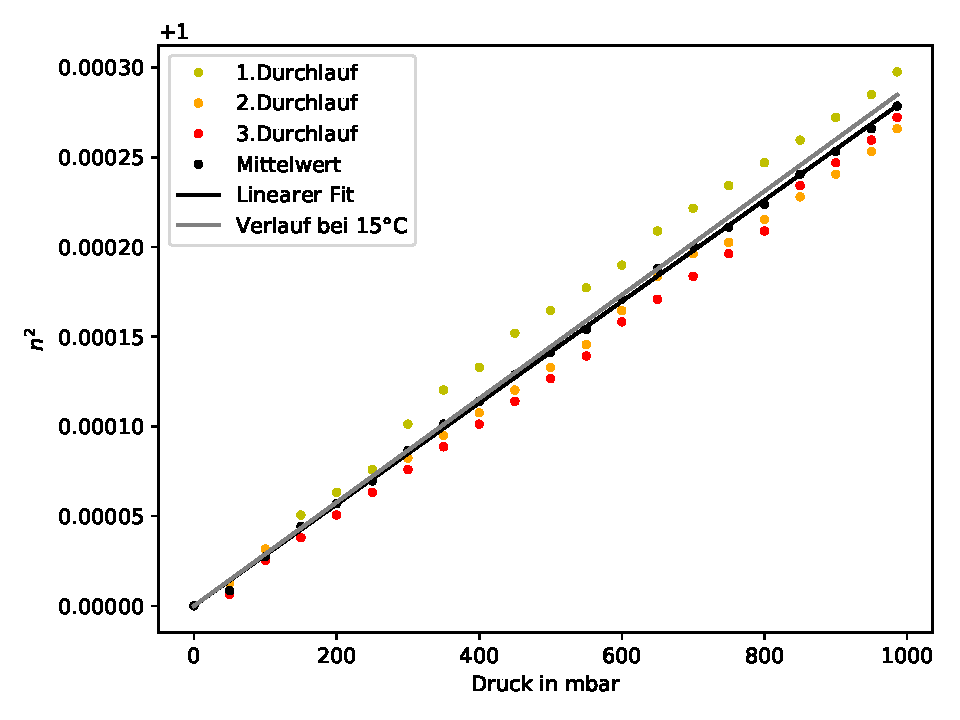
\includegraphics{druck.pdf}
                \caption{Zusammenhang zwischen Druck und Brechungsindex von Luft.}
                \label{fig:luft}
            \end{figure}
            
            Der Mittelwert wird mithilfe der Formel 

            \begin{align*}
                n^2 = c\cdot p + 1
            \end{align*}

            linear gefittet, wobei sich für die Steigung der Geraden

            \begin{align*}
                c = (2,827\pm 0.008)\,10^{-7}\,\symup{mbar}
            \end{align*}

            ergibt. Da die Messungen bei einer Durchschnittlichen Temperatur von 21,2° durchgeführt 
            wurden, ist die Kurve für genau diese Temperatur gültig.
            Ebenfalls in Abb. \ref{fig:luft} ist die entsprechende Gerade für eine Temperatur von 
            15° zu sehen. Aus ihr lässt sich für einen Druck von 1.013\,bar ein Brechungsindex von 

            \begin{align*}
                n_{Luft} \approx 1,00015
            \end{align*}

            berechnen.
